\documentclass[final,hyperref={pdfpagelabels=false},mathserif]{beamer}
\usepackage[]{color}
\usepackage{pdfcolmk}
\usepackage{eulervm}
\usepackage{tikz}
\usepackage{rotating}
\usepackage[scaled]{helvet}
\usepackage{epstopdf}
\usepackage{physics}
\usepackage{pgfplots}
\pgfplotsset{compat=1.8}
\usepackage[table]{colortbl} % table cell colours
\usepackage{hyperref}
\usepackage{graphicx} % Allows including images
\usepackage{booktabs} % Allows the use of \toprule, \midrule and \bottomrule in tables
\usepackage{physics}
\usepackage{tikz}
\usepackage{pgfpages}
\usepackage{caption}
\usepackage{float} % for [H] placement
\usepackage{enumitem}
\usepackage{tcolorbox}
\usepackage[acronym,indexonlyfirst,nomain,nohypertypes={acronym,notation}]{glossaries}
\usepackage{tikz}
\usepackage{chemfig}

%\usepackage[cmbright]{sfmath}
\mode<presentation>
  {
  \usetheme{ChR}
  \setbeamertemplate{bibliography item}[text]
}
  \usepackage{amsmath,amsthm, amssymb, latexsym}
  %\boldmath
  \usepackage[english]{babel}
  \usepackage[utf8x]{inputenc}
  \usepackage[orientation=portrait,size=a0,scale=1.3,debug]{beamerposter}

  % user defined
\newtheorem*{ans}{Ansatz}
\newcommand{\e}{\varepsilon}
\newcommand{\mathbox}[2]{
    \begin{beamercolorbox}[wd=\textwidth,rounded=true,shadow=true,left]{mathbox title}
        \textbf{#1}
    \end{beamercolorbox}

    \begin{beamercolorbox}[wd=\textwidth,rounded=true,shadow=true,left]{mathbox body}
        #2
    \end{beamercolorbox}
}
%  \renewcommand{\arraystretch}{0.7}
  \setlength{\parindent}{0 pt}
  \setlength{\parskip}{0 pt}

  \usepackage{booktabs}
  \renewcommand{\arraystretch}{1}
  \usepackage{array}
  % um Tabellenspalten mit Flattersatz zu setzen, muss \\ vor
  % (z.B.) \raggedright geschuetzt werden:
  \newcommand{\PreserveBackslash}[1]{\let\temp=\\#1\let\\=\temp}
  \newcolumntype{L}[1]{%
    >{\PreserveBackslash\raggedright\hspace{0pt}}p{#1}%
  }
  \usepackage[subfigure]{ccaption}
  \usepackage[FIGBOTCAP]{subfigure}
  \usepackage{multicol}
\usepackage{achemso}
\usepackage{caption}
\captionsetup{font=scriptsize,labelfont=scriptsize}
\setbeamertemplate{caption}[numbered]
\usetikzlibrary{calc,positioning,shapes.geometric,shapes.symbols,shapes.misc,calc,arrows,decorations.pathmorphing,intersections,decorations.pathreplacing,calligraphy}

\usetikzlibrary{decorations.pathreplacing}
\tikzset{
mybrace/.style={decorate,decoration={brace,aspect=#1}}
}
\newcommand*{\citen}[1]{%
  \begingroup
    \romannumeral-`\x % remove space at the beginning of \setcitestyle
    \setcitestyle{numbers,square}%
    \cite{#1}%
  \endgroup
}

%%%%%%%%%%%%%%%%%%%%%%%%%%%%%%%%%%%%%%%%%%%%%%%%%%%%%%%%%%%%%%%%%%%%%%%%%%%%%%%%%5
\graphicspath{{figures/}}
\title{Variational Quantum Nuclear-Electronic Dynamics: \\Proton Transfer on Quantum Computers}
\author{\underline{Dilhan Manawadu}, Edoardo Altamura}
\institute{The Hartree Centre, STFC, Sci-Tech Daresbury, Warrington WA4 4AD, United Kingdom}
  %%%%%%%%%%%%%%%%%%%%%%%%%%%%%%%%%%%%%%%%%%%%%%%%%%%%%%%%%%%%%%%%%%%%%%%%%%%%%%%%%5
  %% sensible column widths: 81cm (1 column);
  %%%%%%%%%%%%%%%%%%%%%%%%%%%%%%%%%%%%%%%%%%%%%%%%%%%%%%%%%%%%%%%%%%%%%%%%%%%%%%%%%5

\newacronym{NEO}{NEO}{Nuclear-Electronic Orbital}
\newacronym{NEOHF}{NEOHF}{NEO Hartree-Fock}
\newacronym{NEOCASCI}{NEOCASCI}{NEO Complete Active Space Configuration Interaction}
\newacronym{UCC}{UCC}{Unitary Coupled Cluster}
\newacronym{QPE}{QPE}{Quantum Phase Estimation}
\newacronym{ADAPT-VQE}{ADAPT-VQE}{Adaptive Derivative-Assembled Pseudo-Trotter Ansatz Variational Quantum Eigensolver}
\newacronym{ADAPT-AQC}{ADAPT-AQC}{Adaptive Approximate Circuit Compilation}
\newacronym{FNO}{FNO}{Frozen Natural orbital}
\newacronym{ZNE}{ZNE}{Zero Noise Extrapolation}
\newacronym{TDSE}{TDSE}{Time-Dependent Schr\"odinger Equation}


\begin{document}
\vskip-1.4cm
%
% Übergeordnete Spalten
%
\begin{columns}[t]
%
% Spalte (1/3 der Seite) für Introduction, Experimental and Methods
% 
\begin{column}{40cm}
      
%
% Introduction 
%
\begin{block}{Quantum effects of proton transfer}

\begin{itemize}[label=\textbullet, leftmargin=1em]

\item Proton transfer reactions are ubiquitous in many chemical and biological processes.
\item Accurate description of proton transfer requires a quantum description of the kinetic nuclei that captures quantum tunnelling and zero-point energy.
\item Several theoretical approaches to accurately model proton transfer like ring polymer molecular dynamics \citen{habershonRingPolymerMolecularDynamics2013} and multi-configuration time-dependent Hartree \citen{beckMulticonfigurationTimeDependentHartree2000} have been developed, however they exhibit prohibitive scaling with the system size.

\end{itemize}

\end{block}

\begin{block}{\gls{NEO} Theory}

\begin{itemize}[label=\textbullet, leftmargin=1em]

\item \gls{NEO} approach solves the mixed nuclear-electronic time-independent Schr\"odinger equation by constructing a mixed nuclear-electronic wavefunction \citen{webb2002multiconfigurational}.

\item \gls{NEO} framework has be complemented with existing electronic structure methods at different levels of theory like \gls{NEOHF} and \gls{NEOCASCI} \citen{pavosevic2020chemrev}.

\item These, however, still suffer from the scalability limitations of the underlying electronic structure methods.

\end{itemize}

\end{block}

\begin{block}{\gls{NEO} approach for modelling proton transfer}

\begin{itemize}[label=\textbullet, leftmargin=1em]

\item \gls{NEO} framework has been extended for implementation on quantum hardware \citen{pavosevicMulticomponentUnitaryCoupled2021a}. 


\item Kovyrshin \textit{et al.} utilised \gls{NEO} framework with the \gls{UCC} ansatz to calculate the energy barrier of proton transfer in malonaldehyde \citen{kovyrshin2023quantum}.

\item This work demonstrated that \gls{NEO} with \gls{UCC} singlets and doublets could reach energy barrier predicted by \gls{NEOCASCI} to within $10^{-4}$ Hartree.

\item Electronic-only CASCI calculation overestimates the barrier of proton transfer, which emphasises the importance of electron-nuclear correlation

\noindent
\begin{minipage}[t]{0.47\textwidth}
\vspace{-5pt} % Ensures top alignment
    \centering
    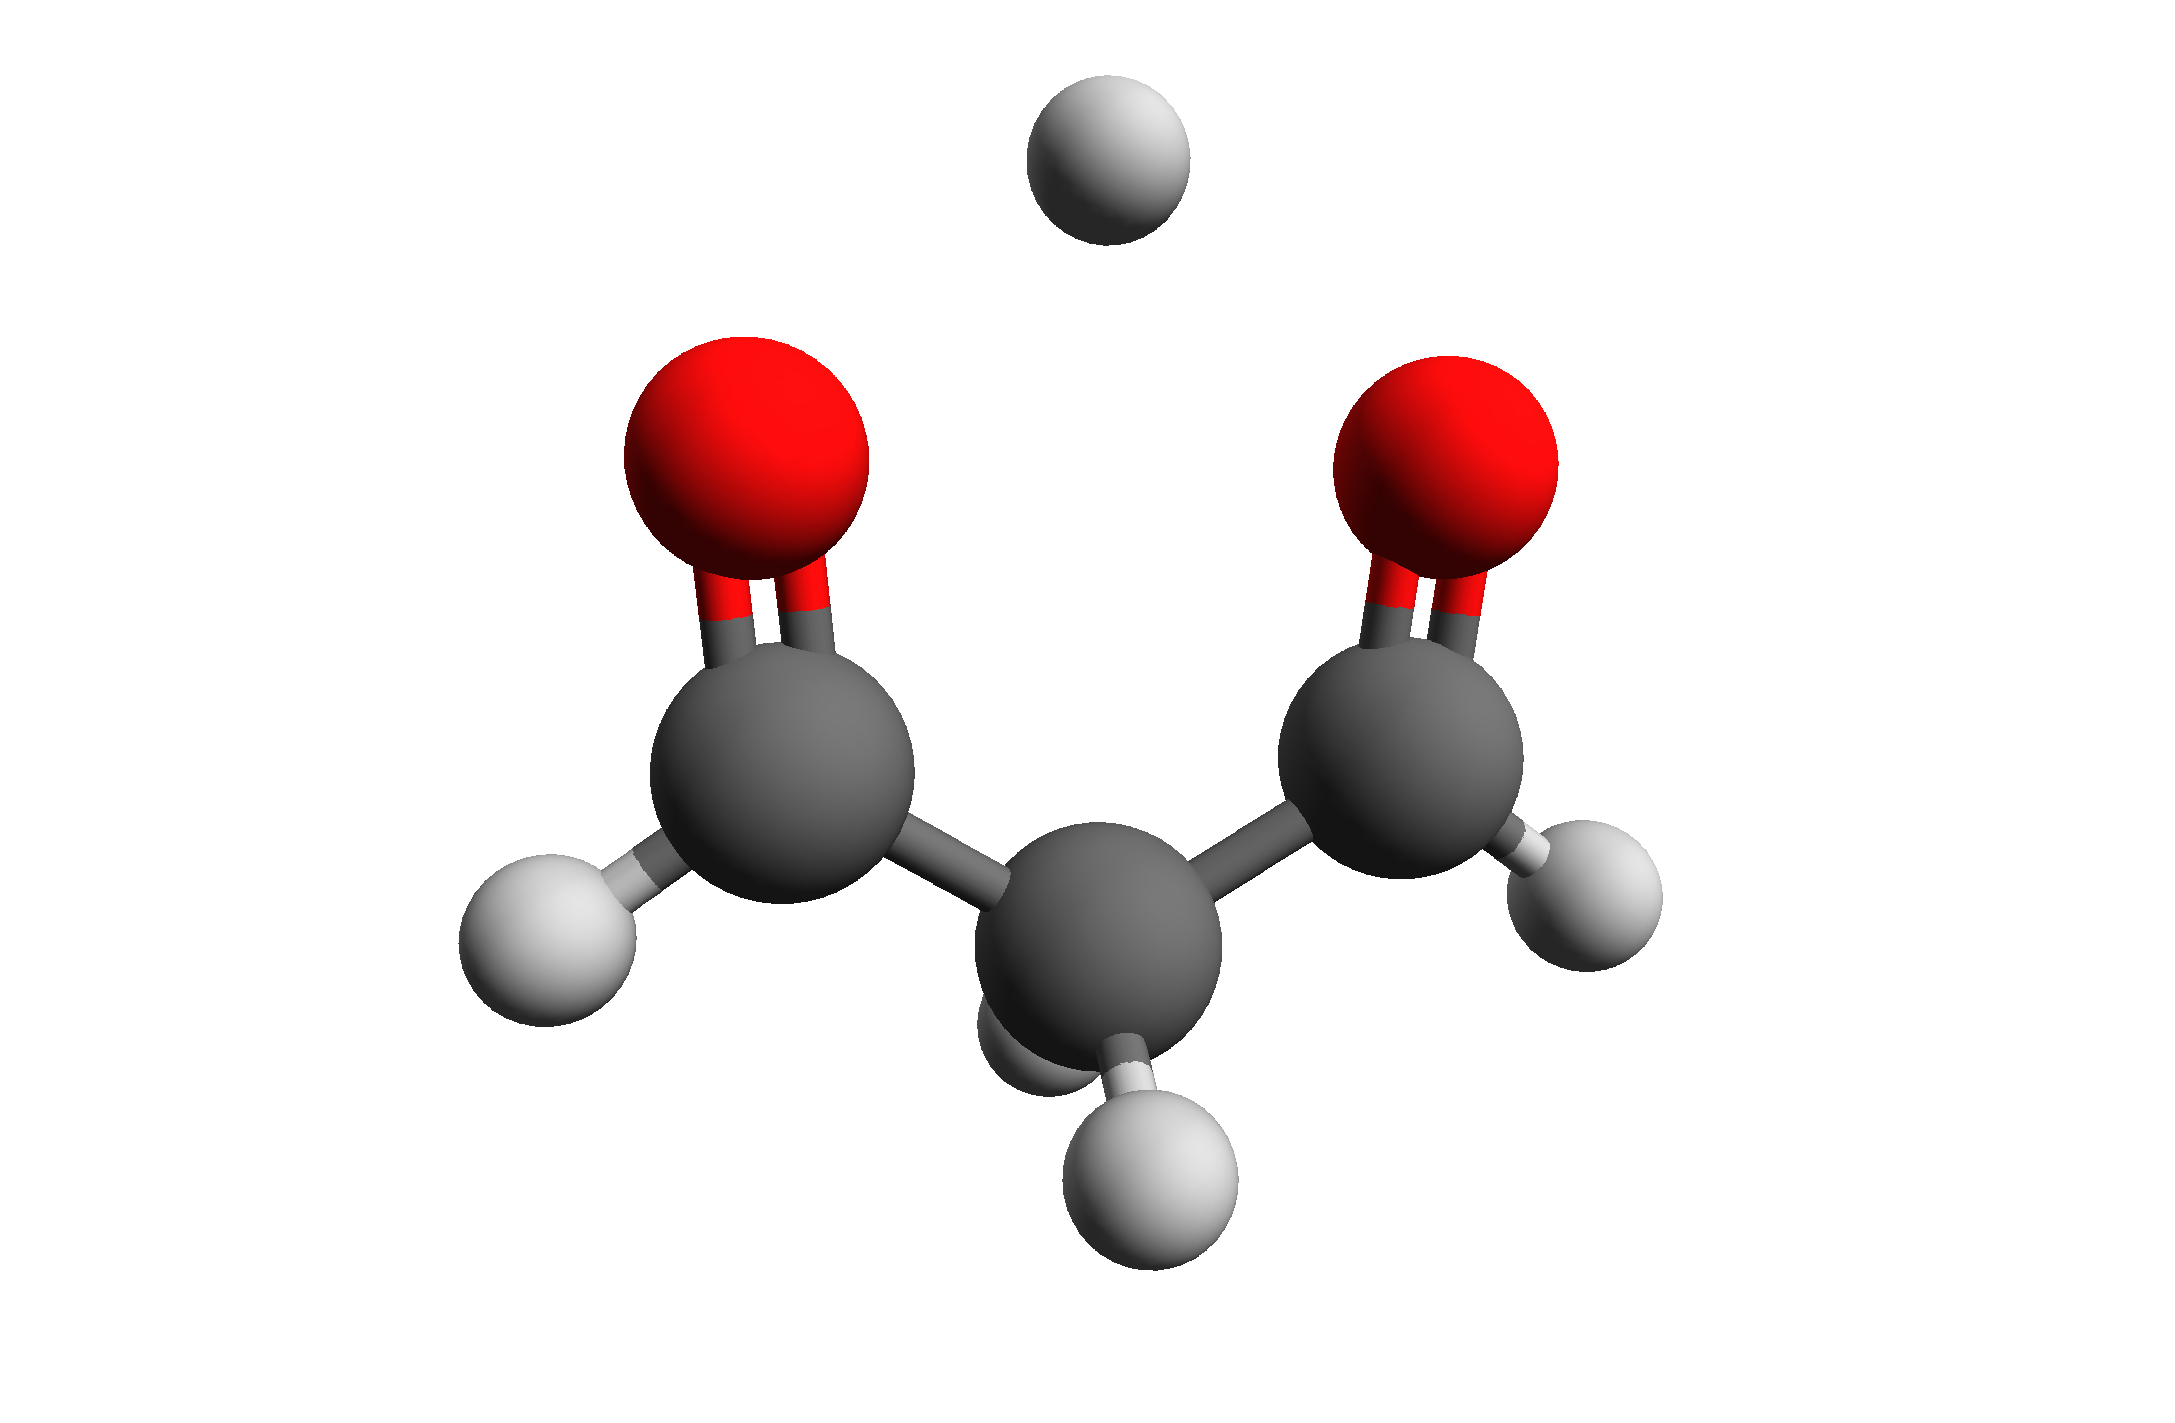
\includegraphics[width=\linewidth]{figures/mal.pdf}
    \captionof{figure}{Chemical structure of malonaldehyde}
\end{minipage}%
\hfill
\begin{minipage}[t]{0.47\textwidth}
\vspace{30pt} % Ensures top alignment
    \centering
    \rowcolors{2}{lightgray}{white}
   \begin{tabular}{|
        >{\columncolor{oxford-blue}\color{white}\hspace{6pt}}c<{\hspace{6pt}}|
        >{\columncolor{oxford-blue}\color{white}\hspace{6pt}}c<{\hspace{6pt}}|}
        \hline
        Method & $\Delta E/\textrm{Ha}$ \\
        \hline
        \rowcolor{gray!10} \color{black}{CASCI} & \color{black}0.011962 \\
        \color{black}\gls{NEOCASCI} & \color{black}0.005011 \\
        \rowcolor{gray!10} \color{black}NEOUCCSD & \color{black}0.004924 \\
        \color{black}NEOUCCSDT & \color{black}0.005007 \\
        \rowcolor{gray!10} \color{black}NEOUCCSDTQ & \color{black}0.005009 \\
        \hline
    \end{tabular}
    \captionof{table}{Barrier for proton transfer in malonaldehyde calculated using different flavours of \gls{NEO}. Values reproduced from Ref. \citen{kovyrshin2023quantum}.}
    
\end{minipage}

\end{itemize}



\end{block}

\begin{block}{Quantum resource reduction using ADAPT-VQE}

\begin{itemize}[label=\textbullet, leftmargin=1em]

\item \gls{NEO} framework with \gls{UCC} ansatze offers a way of modelling proton transfer in polynomial time using the \gls{QPE} \citen{aspuru-guzikSimulatedQuantumComputation2005} algorithm.

\item However, these circuits are too deep to be meaningfully realised on current hardware for chemically interesting systems.

\item Nyk\"anen \textit{et al.} extended the hardware efficient \gls{ADAPT-VQE} for \gls{NEO} framework. This method, titled \gls{FNO}-\gls{NEO}-\gls{ADAPT-VQE} enables high fidelity circuit construction tailored for currently available quantum hardware \citen{nyke2023}.

\item By using a \gls{FNO} basis, they were able to reduce the qubit requirement, while the adaptive ansatze building led to shallower circuits.

\end{itemize}



\end{block}

\begin{block}{Adaptive approximate matrix product state preparation}

\begin{itemize}[label=\textbullet, leftmargin=1em]

\item \gls{ADAPT-AQC}, an adaptive algorithm based on approximate circuit compiling to construct high fidelity shallow circuits that approximates a given quantum circuits was recently proposed by Jadenberg \textit{et al.} \citen{jaderbergVariationalPreparationNormal2025}.

\item In conjunction with \gls{ADAPT-VQE}, this provides a toolbox of implementing quantum circuits to capture proton dynamics of small molecules on currently available quantum hardware.


\end{itemize}

\end{block}

\begin{block}{Approximate quantum compilation of proton-transfer dynamic for quantum processors}
\vspace{-0.4em} % Adjust this value as needed

\begin{tcolorbox}[colframe=blue!50!black, colback=blue!10!white]

\begin{itemize}[label=\textbullet, leftmargin=1em]

\item In this work, we demonstrate a quantum computing pipeline based on \gls{NEO} framework to model proton transfer of malonaldehyde. 

\item We suggest strategies to construct quantum circuits to tailor for current and future quantum hardware.

\item We perform proton transfer barrier estimation simulations using realistic hardware noise models.

\end{itemize}

\end{tcolorbox}
\vspace{-0.2em} % Adjust this value as needed
\end{block}


\end{column}

\begin{column}{40cm}


\begin{block}{Theory}

\begin{itemize}[label=\textbullet, leftmargin=1em]

\item The dynamics of the system is described by the \gls{TDSE}
\begin{equation}
    \label{eq:tdS}
    %i \hbar \frac{\partial}{\partial t} |\Psi(t)\rangle = \left[ T_p + V_p(t) + H_e(t) + H_{ep}(t) \right] |\Psi(t)\rangle
    i \hbar~\frac{\partial}{\partial t} \big|\Psi(t)\big\rangle = \left[ \hat T_p + \hat V(t) \right]~\big|\Psi(t)\big\rangle \, ,
\end{equation}
where $\hat{T}_p$ is the kinetic energy operator for the proton, and $\hat{V}(t)$ is a time-dependent potential given by
\begin{equation}
    \label{eq:Vp}
    \hat V(t) = \hat V_p(t) + \hat V_{ep}(t) + \hat H_e(t) \, 
\end{equation}
where $\hat V_p(t)$ describes the interaction of the proton with the classical nuclear scaffold,
$\hat V_{ep}(t)$ is the proton-electron interaction and  $\hat H_e(t)$ is the electronic Hamiltonian contribution. 
\item We can write the \gls{NEO}CI wavefunction with nuclear and electronic components $\ket{\Phi_{\nu}^n}$ and $\ket{\Phi_{\mu}^e}$ respectively as 
\begin{align}
    \label{eq:neofci}
    \ket{\Psi [\vec{C}(t)]} = \sum_{\mu \nu}C_{\mu \nu}(t) \ket{\Phi_{\mu}^e} \ket{\Phi_{\nu}^n} \, .
\end{align}

\item This leads to an equation of motion for the CI coefficients $\vec{C}(t)$
\begin{equation}\label{eq:motion}
    \vec{H}(t) \vec{C}(t) = i\frac{\partial}{\partial t}\vec{C}(t)\, ,
\end{equation}
where the matrix elements of $\vec{H}(t)$ are defined by
\begin{equation}\label{eq:Ht}
    H_{\kappa \lambda, \mu \nu}(t)=\bra{\Phi^e_{\kappa}}\bra{\Phi^n_{\lambda}} \hat T_p + \hat V(t)\ket{\Phi^e_{\mu}} \ket{\Phi^n_{\nu}} \, .
\end{equation}

\item Previously, Kovyrshin \textit{et al.} explored the dynamics of this model through Suzuki-Trotter decomposition  \citen{kovyrshinNonadiabaticNuclearElectron2023}. This approach is too computationally demanding for current hardware.

\item To make our approach viable with current and near-future hardware, we explore the adiabatic regime of proton transfer by slowly varying the Hamiltonian. At each time step, the energy of the instantaneous proton-electron Hamiltonian is obtained by variationally minimising
\begin{equation}
    \label{eq:AdTr}
    E(t) = \min_{\vec{C}(t)} \frac{\bra{\Psi [\vec{C}(t)]} \hat{T}_p + \hat{V}(t) 
    \ket{\Psi[\vec{C}(t)]}}{\bra{\Psi [\vec{C}(t)]}\ket{\Psi [\vec{C}(t)]}}.
\end{equation}

\end{itemize}

\end{block}







\begin{block}{Pipeline for proton transfer simulation}

\begin{figure}[ht]
\begin{center}
\vspace*{0.5cm}

\begin{tikzpicture}
  % Main node
  \node[draw=oxford-blue, 
        fill=oxford-blue!40, 
        rounded corners, 
        minimum width=4cm, 
        minimum height=1.5cm, 
        text=black] 
  (prep) at (0,0) {NEO-FNO-ADAPT-VQE};

  % Arrow endpoints
  \coordinate (left) at (-8,-3);
  \coordinate (right) at (8,-3);

  % Arrows from center bottom
  \draw[->, ultra thick] (prep.south) -- (left);
  \draw[->, ultra thick] (prep.south) -- (right);

  % Target nodes
  \node[draw=oxford-blue, 
        fill=oxford-blue!10, 
        rounded corners, 
        minimum width=4cm, 
        minimum height=1.5cm, 
        text=black] 
  (deep) at (left) {Deep ADAPT-VQE};

  \node[draw=oxford-blue, 
        fill=oxford-blue!10, 
        rounded corners, 
        minimum width=4cm, 
        minimum height=1.5cm, 
        text=black] 
  (shallow) at (right) {Shallow ADAPT-VQE};

  % Downward arrow from shallow
  \node[draw=oxford-blue, 
        fill=oxford-blue!40, 
        rounded corners, 
        minimum width=4.5cm, 
        minimum height=1.5cm, 
        text=black] 
  (compile) at (8,-6) {Approximate Circuit Compiling};

  \draw[->, ultra thick] (shallow.south) -- (compile.north);

  % New nodes from Approximate Circuit Compiling
  \coordinate (compLeft) at (3,-10);
  \coordinate (compRight) at (13,-10);

  \node[draw=oxford-blue, 
        fill=oxford-blue!10, 
        rounded corners, 
        minimum width=4.5cm, 
        minimum height=1.8cm, 
        align=center,
        text=black] 
  (high) at (compLeft) {High Fidelity\\ADAPT-AQC};

  \node[draw=oxford-blue, 
        fill=oxford-blue!10, 
        rounded corners, 
        minimum width=4.5cm, 
        minimum height=1.8cm, 
        align=center,
        text=black] 
  (low) at (compRight) {Low Fidelity\\ADAPT-AQC};

  % Arrows from Approximate Circuit Compiling
  \draw[->, ultra thick] (compile.south) -- (high.north);
  \draw[->, ultra thick] (compile.south) -- (low.north);

  % Final nodes
  \node[draw=oxford-blue, 
        fill=oxford-blue!50, 
        rounded corners, 
        minimum width=4.8cm, 
        minimum height=1.8cm, 
        align=center,
        text=black] 
  (fault) at (3,-15) {Early Fault\\Tolerant Regime};

  \node[draw=oxford-blue, 
        fill=oxford-blue!50, 
        rounded corners, 
        minimum width=4.8cm, 
        minimum height=1.8cm, 
        align=center,
        text=black] 
  (noisy) at (13,-15) {Noisy Simulations\\(IBM Fez)};

  % Arrows from AQC nodes
  \draw[->, ultra thick] (high.south) -- (fault.north);
  \draw[->, ultra thick] (low.south) -- (noisy.north);

\end{tikzpicture}

\end{center}

\caption{Starting with a variationally optimised \gls{FNO}-\gls{NEO}-\gls{ADAPT-VQE} ansatz, we generate two sets of \gls{ADAPT-VQE} circuits using different convergence thresholds. These are further truncated via \gls{ADAPT-AQC} to optimise the circuit depth. Deeper circuits are simulated without noise to emulate early fault tolerance, while shallower ones are simulated on the noisy IBM Fez model with \gls{ZNE}.}
\label{fig:neo-fno-adapt-vqe}
\end{figure}


\end{block}

\begin{block}
{Results}
\centering
Soon to be published!

\end{block}

%
% Introduction 
%
\begin{block}
{Acknowledgements}

This work was supported by the Hartree National Centre for Digital Innovation, a UK Government-funded collaboration between STFC and IBM.
\end{block}

\begin{block}{References}
\scriptsize
\rightskip=0pt plus 1pt
\hyphenpenalty=10000

\bibliography{/Users/dilhan.manawadu/Writing/Bibliography/WATOC2025}
\end{block}
\end{column}

\end{columns}

% Ende Poster Seite und Dokument!
%
\end{document}